% !TEX TS-program = pdflatex
% !TEX encoding = UTF-8 Unicode
% !TEX root = ../main.tex
% !TEX spellcheck = en-US
% ****************************************************************************************
% File: func_descr_and_theor_aspects.tex
% Author: Patrick Haselwanter, Christoph Ehrhardt
% Date: 2023-10-28
% ****************************************************************************************
\chapter{Meshing of the Domain}
\label{chapter:meshing}

The meshing of the domain is a crucial step in the simulation process as it directly affects the accuracy of the results. 
The following settings were used:
\begin{itemize}
    \item item size of \qty{2}{\milli\meter}
    \item 5 inflation layers with growth rate 1,2
\end{itemize}

The mesh of the whole domain for the basic geometry is shwon in \autoref{fig:meshing_base_geometry_full_view} while \autoref{fig:meshing_base_geometry_detailed_view} shows a detailed view of the meshing at the walls and heater element.


\begin{figure}[htbp]   
    \centering
    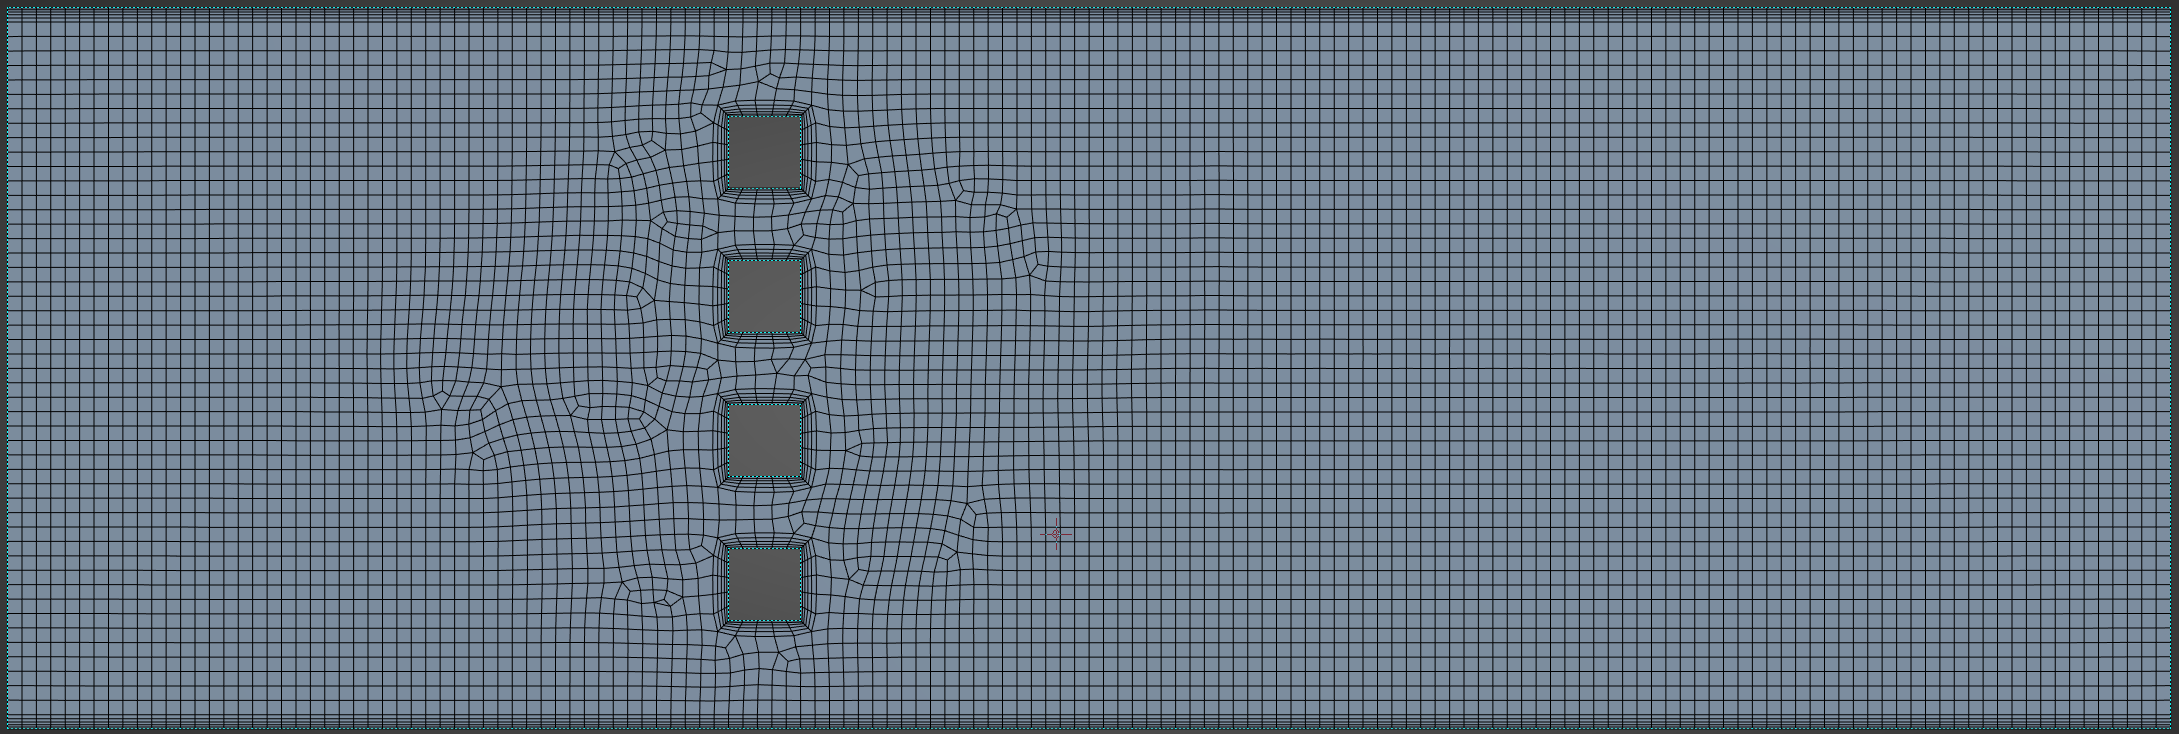
\includegraphics[width=0.8\textwidth]{img/meshing_base_geometry_full_view}
    \caption{Full view of the base geometry meshing}
    \label{fig:meshing_base_geometry_full_view}
\end{figure}


\begin{figure}[htbp]
    \centering
    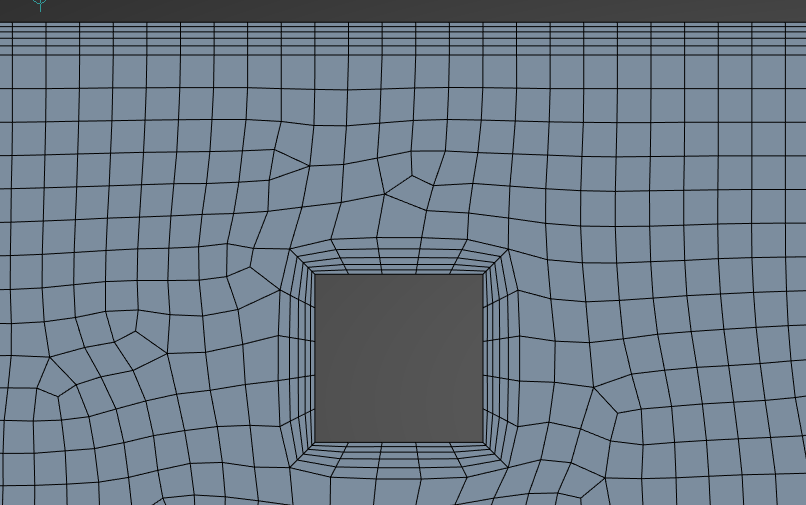
\includegraphics[width=0.8\textwidth]{img/meshing_base_geometry_detailed_view}
    \caption{Detailed view of the base geometry meshing}
    \label{fig:meshing_base_geometry_detailed_view}
\end{figure}

\section{Grid Convergence Study}
\label{sec:grid_convergence_study}

To ensure the mesh independency of the results, a grid convergence study according to \autocite{ExaminingSpatialGrid} was performed.
The mesh size was varied between \qty{4}{\milli\meter}, \qty{2}{\milli\meter} and \qty{1}{\milli\meter} whilst keeping the number of inflation layers constant. To evaluate the results, the area-weighted average static temperature across the flow \qty{25}{\milli\meter} before the outlet was used.
The results are shown in \autoref{tab:grid_convergence_study} and \autoref{fig:grid_convergence_graph}.

\begin{table}[htbp]
    \centering
    \caption{Grid convergence study}
    \label{tab:grid_convergence_study}
    \begin{tabular}{lcc}
        \toprule
        Mesh size & Temperature [\unit{\kelvin}] \\
        \midrule
        \qty{4}{\milli\meter} & 305.62 \\
        \qty{2}{\milli\meter} & 304.96 \\
        \qty{1}{\milli\meter} & 304.69 \\
        Richardson Extrapolation & 304.503 \\
        \bottomrule
    \end{tabular}
\end{table}

\begin{figure}
    \centering
    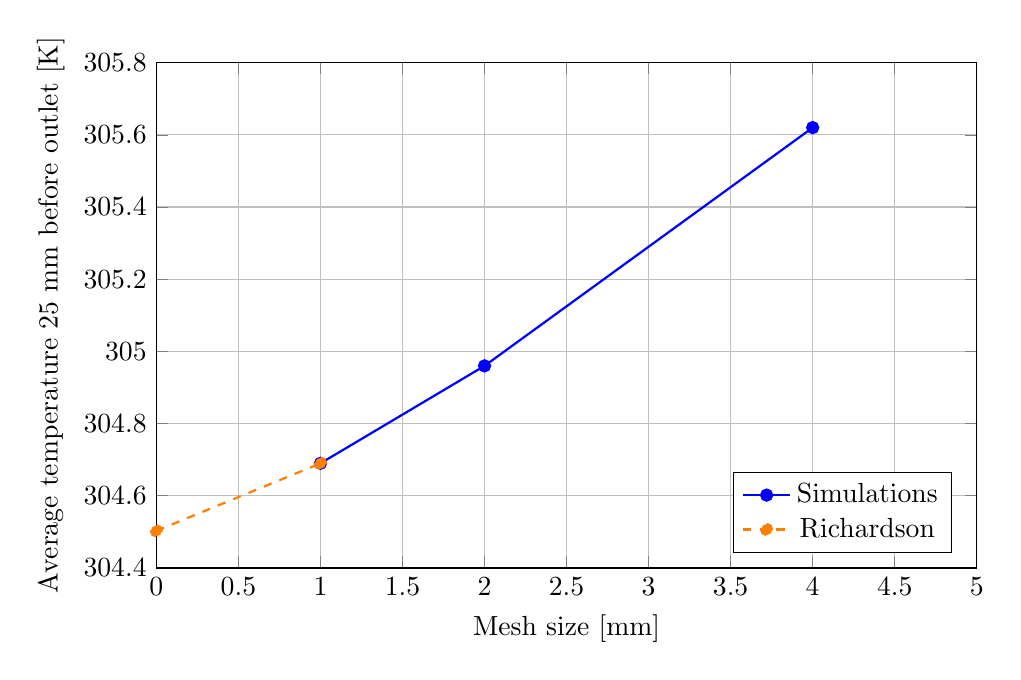
\begin{tikzpicture}
        \begin{axis}[
            width=12cm, height=8cm,
            xlabel={Mesh size [mm]},
            ylabel={Average temperature 25 mm before outlet [K]},
            legend pos=south east,
            grid=both,
            xmin=0, xmax=5,
            ymin=304.4, ymax=305.8
        ]
            % Simulations data
            \addplot[color=blue, mark=*, thick] coordinates {
                (1, 304.69)
                (2, 304.96)
                (4, 305.62)
            };
            \addlegendentry{Simulations}

            % Richardson extrapolation data
            \addplot[color=orange, dashed, mark=*, thick] coordinates {
                (0, 304.503)
                (1, 304.69)
            };
            \addlegendentry{Richardson}
            
        \end{axis}
    \end{tikzpicture}
    \caption{Grid convergence graph showing the variation of temperature with mesh size}
    \label{fig:grid_convergence_graph}
\end{figure}

The grid convergence study yields an asymptotic range of convergence of 0.99911, a \qty{0.19}{\percent} \gls{acr:gci} between \qty{4}{\milli\meter} and \qty{2}{\milli\meter} and a \qty{0.08}{\percent} \GLS{acr:gci} between \qty{2}{\milli\meter} and \qty{1}{\milli\meter} mesh sizing and thus shows that the results can be seen as mesh independent for a mesh size of \qty{2}{\milli\meter}.


% EOF